\appendix
\section{Observe the impact of scheduled positive events: students' stress during exam intervals in two situations}
\begin{table*}
\begin{center}
\caption{\small{Algorithm 1: Select candidate stress intervals impacted by positive events.}}
\begin{tabular}{l} \hline
A candidate interval $I = <w_1,\cdots, w_i,\cdots, w_m>$ is identified with following rules:\\
\textcircled{1} $s^{'}_1 = 0$, $s^{'}_m = 0$. $\forall s^{'}_j \in \{s^{'}_2,\cdots,s^{'}_{m-1}\}$, $s^{'}_j > 0$.\\
\textcircled{2} Let $w_i$ be the biggest wave in current candidate interval, with $peak(w_i) = \omega$, $\forall $ wave $w_j \in I$, $peak(w_j)<=peak(w_i)$.\\
\textcircled{3} For $w_k$ before the interval biggest wave $w_i$ , i.e., $\forall w_k \in <w_1,\cdots,w_{i-1}>$, $peak(w_{k+1})>=peak(w_k)$, $vally(w_{k+1}) >= peak(w_k)$.\\
\textcircled{4} For $w_k$ behind the interval biggest wave $w_i$, i.e.,  $w_k \in <w_{i}, \cdots, w_m>$, $peak(w_{k+1})<=peak(w_k)$, $vally(w_{k+1}) <= peak(w_k)$.\\\hline
\end{tabular}
\end{center}
\end{table*}

\begin{figure}
\centering
\caption{Compare students' stress during exam intervals in two situations:
1) affected by neighboring uplift events (U-SI), 2) no uplift events occurred nearby (SI)}
\includegraphics[width=\linewidth]{figs/frequency.eps}
\label{fig:frequency}
\end{figure}

To further observe the influence of uplift events for students facing stressor events,
we statistic all the stressful intervals~\cite{Li2017Analyzing} detected surround the scheduled examinations over the 124 students during their high school career.
For each student, we divide all his/her stressful intervals into two sets:
1) stressful intervals under the influence of neighbouring uplift events (e.g., \emph{Halloween activity}), and 2) independent stressful intervals.
Figure~\ref{fig:frequency} shows five measures of each student during the above two conditions:
the \emph{accumulated stress}, the \emph{average stress} (per day), the \emph{length of stressful intervals},
the \emph{frequency of academic topic words}, and the \emph{ratio of academic stress among all types of stress}.
For each measure, we calculate the average value over all eligible slides for each student.

\section{Algorithm 1: Select candidate intervals impacted by positive events}
\label{alg:alg1}
Let the sub-series $w_{<a,b>} = [s^{'}_a, \cdots, s^{'}_b]$ as a \emph{wave},
where $s^{'}_v$ $= {vally(w_{<a,b>})}$ is the minimum stress value,
$s^{'}_p$ $= peak(w_{<a,b>})$ is the maximal stress value during $\{s^{'}_a,\cdots,s^{'}_b\}$,
and $s^{'}_a \leq s^{'}_{a+1} \leq \cdots \leq s^{'}_p \leq s^{'}_{p+1} \leq \cdots \leq s^{'}_b$.

\section{Algorithm2: Identify stressful intervals impacted by positive events.}
\label{alg:alg2}
For each candidate interval,
a Poisson based probability model~\cite{Li2017Analyzing} is adopted to measure how confidently the current interval is a stressful interval.
Here a teen's stressful posting rate under stress ($\lambda_1$) and normal conditions ($\lambda_0$) are modeled as two independent poisson process:
\begin{equation}
Pr[N=n|\lambda_i]=\frac{e^{-\lambda_i T}{(\lambda_i T)}^n}{n!}
\end{equation}
where $i\in\{0,1\}$, $n=0,1,\cdots,\infty$.
We expect that $\lambda_1 > \lambda_0$, and measure the probability as $P(\lambda_1>\lambda_0|N_1, T_1, N_0, T_0)$,
where $N_1, N_0$ are the number of stressful posts, and $T_1, T_0$ are time duration corresponding to $\lambda_1$ and $\lambda_0$.
Without loss of generality, we assume a Jeffreys non-informative prior on $\lambda_1$ and $\lambda_0$,
and infer the posterior distribution $P(\lambda_1|N_1)$ and $P(\lambda_0|N_0)$ according to Bayes Rule.
Thus for current interval $I_1$ and historical normal interval $I_0$,
the quantified probability $\beta = P(\lambda_1>\lambda_0|I_1,I_0)$ $\in (0,1)$ indicates the confidence whether $I_1$ is a stressful interval.


\section{Algorithm3: judge stressful intervals into SI or U-SI}
\label{alg:alg3}
In this part, we filter out two sets of stressful intervals: stressful intervals without the impact of uplift events (SI),
and stressful intervals under the impact of uplift events (U-SI).
For a detected stressful interval $I = <t_1,\cdots,t_n>$, we consider the temporal order between $I$ and any detected uplift event $u$ happened at time point $t_u$:
\begin{itemize}
\item If the uplift event $u$ happens during the stressful interval, i.e., $t_u \in [t_1,t_n]$, the uplift interval $I$ is judged as $I \in SI$.
\item For the uplift event happening nearby a stressful interval,
we also consider the probability that it conducts impact on the teen's stressful interval.
Here the gap between $t_u$ and $I$ is limited to $\xi$, i.e.,
if $t_u \in [t_{1}-\xi, t_1)\cup(t_{n},t_{n}+\xi]$, then $I \in SI$.
%The setting of parameter $\xi$ is discussed in experiment section.
\end{itemize}
If a stressful interval satisfies none of the above conditions, we classify it into the U-SI set.

\subsection{Model 1: quantify significant restoring impact conducted by uplift events}
\label{mod:mod1}
For each teen, three groups of behavioral measures are considered: \emph{posting behavior},
\emph{stress intensity} and \emph{linguistic expressions},
indicated as \bm{${<D_p}$},\bm{${D_s}$},\bm{${D_l>}$}, respectively.
To measure the correlation for each group of positive and stressful behavioral measures,
the Euclidean distance is adopted to calculate the distance of structured points in $A_1$ and $A_2$.

For each point $\ell x \in A=A_1\bigcup A_2$,
let $NN_r(\ell_x,A)$ be the function to find the $r-$th nearest neighbor of $\ell_x$.
Specifically, according to the three group of measures,
three sub-functions of $NN_r(.)$ are defined as $PNN_r(.)$, $SNN_r(.)$ and $LNN_r(.)$,
corresponding to the teen's posting behaviors, stress intensity and linguistic expressions in each stressful interval,  respectively.

For point $\ell_x$ with posting behavior matrix \bm{${D_p^x}$}, stress intensity matrix \bm{${D_s^x}$},
and linguistic expression matrix \bm{${D_l^x}$},
the $r$-th nearest neighbor of $\ell_x$ in each measure is denoted as:
\begin{equation}
\begin{aligned}
& PNN_r(\ell_x,A)
= \{y | min\{||\textbf{D}_p^x-\textbf{D}_p^y ||_2\}, y\in(A/\ell_x)\} &\\
& SNN_r(\ell_x,A)
= \{z | min\{||\textbf{D}_s^x-\textbf{D}_s^z ||_2\}, z\in(A/\ell_x)\} \\
& LNN_r(\ell_x,A)
= \{w | min\{||\textbf{D}_l^x-\textbf{D}_l^w ||_2\}, w\in(A/\ell_x)\} &
 \end{aligned}
 \end{equation}
The $r$-th nearest neighbor considering all three groups of measures is denoted as:
\begin{align}
&NN_r(\ell_x,A) = \{v | min\{a \times ||\textbf{D}_p^x-\textbf{D}_p^v||_2+\\
&b \times ||\textbf{D}_s^x-\textbf{D}_s^v||_2+
c \times ||\textbf{D}_l^x-\textbf{D}_l^v||_2\}, v\in(A/\ell_x) \}
\end{align}
In this study, we set $a = b = c = 1/3$.
Next, let $I_r(\ell_x,A1,A2)$ be the function denoting whether the $r$-th nearest neighbor is in the same set with $\ell_x$:
\begin{equation}
I_r(\ell_x,A_1,A_2) =
\left\{ \begin{array}{ll}
1, \quad if \ell_x \in A_i  \&\& NN_r(\ell_x,A)\in A_i,\\
0, \quad otherwise
\end{array}
\right.
\end{equation}
Let $T_{r,n}$ denote the proportion that pairs containing two points from the same set among all pairs formed by $\ell_x \in A$
and its $k$ nearest neighbors:
\begin{equation}
T_{k,n}= \frac{1}{n\times k}\sum_{i=1}^{n}\sum_{j=1}^{k}I_j(x,A_1,A_2)
\end{equation}
The value of $T_{k,n}$ shows how differently the points in the two testing sets (SI and U-SI) perform in three groups of measures.
If the value of $T_{r,n}$ is close to $1$,
it can be shown that the two underlying distributions $F^{(1)}$ and $F^{(2)}$ for $SI$ and U-SI are significantly different,
indicating current uplift events conduct obvious restoring impact on the teens' stress series.
Let $\lambda_1=|A_1|$ and $\lambda_2=|A_2|$, the statistic value $Z$ is denoted as:
\begin{align}
&Z=(nr)^{1/2}(T_{r,n}-\mu_{r})/\sigma_{r}\\
&\mu_r=(\lambda_1)^2+(\lambda_2)^2\\
&{\sigma_r}^2=\lambda_1\lambda_2+4{\lambda_1}^2{\lambda_2}^2
\end{align}
where $\mu_r$ is the expectation and ${\sigma_r}^2$ is the variance of $Z$.
Based on hypothesis test theory \cite{Johnson2012Applied},
when the size of the testing set ($\lambda_1$ and $\lambda_2$) are large enough,
$Z$ obeys a standard Gaussian distribution.

Thus we judge whether the uplift events have conducted significant restoring impact on the teen's stress series as follows:
if $f(SI,USI)=(nr)^{1/2}(T_{r,n}-\mu_{r})/{\mu_r}^2>\alpha$ ($\alpha = 1.96$ for $P=0.025$),
then the hypothesis $H_1$ is true.

%-----------------------------------------
\section{Model2: identify the temporal order of stress-restoring impact}
\label{mod:mod2}
For a stressful interval $I = <t_i,t_{i+1},\cdots,t_j>$,
let $I^{front} = <t_m,\cdots,t_{i-1}>$ be the adjacent interval before $I$,
and $I^{rear} = <t_{j+1},\cdots,t_n>$ be the rear adjacent interval of $I$.
The length of $I^{front}$ and $I^{rear}$ are set to $|I|$.
For the set of stressful intervals $SI$ composed of $<I_1,I_2,\cdots,I_N>$,
the corresponding sets of adjacent front and rear intervals are denoted as $SI^{front}$ and $SI^{rear}$.
Similarly, for the set of stressful intervals $U-SI$ = $<UI_1,UI_2,\cdots, UI_M>$ impacted by uplift events,
the corresponding sets of adjacent front and rear intervals are denoted as $USI^{front}$ and $USI^{rear}$.
We compare the intensity of stress changes in following four situations,
where $g(.)$ is the function comparing two sets.

\begin{itemize}
\item[\textcircled{1}] $g(SI,SI^{front}$) returns if intensive change happens when stressful intervals begin.
\item[\textcircled{2}] $g(SI,SI^{rear}$) returns if the teen's stress change intensively after the stressful intervals end.
\item[\textcircled{3}] $g(USI,USI^{front}$) returns if intensive change happens when stressful intervals affected by uplift events appears.
\item[\textcircled{4}] $g(USI,USI^{rear}$) returns if stress change intensively after stressful intervals affected by uplift events end.
\end{itemize}

In our problem, taking the comparison between $SI$ and $SI^{rear}$ for example,
the basic computation element $I_k \in SI \cup SI^{rear}$ in both sets is a multi-dimension interval.
Here we adopt the t-test method as the intensity computation function $g(.)$.
The t-test algorithm measures if intensive positive or negative monotonous correlation
exists between two sample sets.
The function $g(.) = t_{score}$ $\in$ (-1,1) is represented as:

\begin{equation}
\small{g(SI,SI^{rear})}= \frac{\mu_{SI}-\mu_{SI^{rear}}}{\sqrt{\frac{(n_1-1)\sigma^2_{SI}+(n_2-1)\sigma^2_{SI^{rear}}}{n_1+n_2-2}(\frac{1}{n_1}-\frac{1}{n_2})}}
\end{equation}
where $\mu_{SI}$ and $\mu_{SI^{rear}}$ are the mean stress values of intervals in sets $SI$ and $SI^{rear}$,
and $\sigma_{SI}$ and $\sigma_{SI^{rear}}$ are the variance stress values of intervals in sets $SI$ and $SI^{rear}$, respectively.
If $g(SI,SI^{rear})$ $> \alpha$, stress intensity in $SI^{rear}$ show significant decrease compared with $SI$ (monotonic negative effect).
If $g(SI^{front},SI)$ $< -\alpha$, stress intensity in $SI$ show significant increase compared with $SI^{front}$ (monotonic positive effect).
Here we adopt $\alpha$ = 1.96, $P$ = 0.025.
We conduct comparison for above four situations,
to observe whether the occurrence of uplift events relieve the monotonic negative effect of $g(SI,SI^{rear})$
and the monotonic positive effect of $g(SI^{front},SI)$.

\section{Algorithm4: Overall algorithm}
\label{alg:alg4}
The overall pipeline for identifying the restoring impact of uplift events is presented here.
1) To quantify the restoring impact of uplift events,
we first extract uplift events and stressful intervals from the teen's microblogs.
All stressful intervals are classified into two sets:
the set of stressful intervals affected by uplift events (SI),
and the set of stressful intervals impacted by uplift events (U-SI).
2) To judge if SI are statistically different with U-SI,
next, the two-sample hypothesis testing method is conducted on the two sets
with multi positive and stressful measures (posting behavior, stress intensity and linguistic expressions).
3) To further judge the monotonous restoring intensity of each type of uplift events,
the final step comes to comparing SI and U-SI with adjacent intervals, respect to temporal order.

For an uplift event $u$ with type $U'$,
a stressor event $e$ with type $S'$,
the overall algorithm is represented as
$F: (u, U', e, S')$ $\rightarrow$ \bm{${A}$}.

{\footnotesize%\small
\begin{algorithm}
  \caption{Identify the restoring impact of uplift events.}
  \label{alg:quantify}
  \KwIn{
  SI: Set of stressful intervals caused by $S'$; \\
  \quad \quad \quad \, U-SI: Set of stressful intervals affected by $U'$;}
  \KwOut{Restoring impact of uplift $U'$ on stressor $S'$: \bm{${A}$}}
  \textbf{Initialize:}  $H_1, H^{front}, H^{rear} = false$;\\
  \If{$f(SI,USI) >$ $\alpha$} {$H_1 = ture$;}
  \If{   $g(SI,SI^{rear}$) $> \alpha$ \&\& $g(SI,SI^{rear}$) $> g(USI, USI^{rear}$)}
  {
  	$H^{rear} = true;$
  }
  \If{$g(SI^{front},SI)$ $< -\alpha$ \&\&  $g(SI,SI^{front}$) $< g(USI, USI^{front}$)}
  {
  	$H^{front} = true;$
  }
  \Return \bm{${A}$} = $<H_1, H^{front}, H^{rear}>$;
\end{algorithm}
}
